%-------------------------------------------------------------------------------
% 								BAB I
% 							LATAR BELAKANG
%-------------------------------------------------------------------------------

\chapter{PENDAHULUAN}

\section{Latar Belakang}
Gas LPG 3 Kg sekarang telah menjadi kebutuhan utama bagi masyarakat di Indonesia sejak pemerintah melakukan konversi dari minyak tanah ke LPG (\textit{Liquified Petroleum Gas}) 3 kilogram (Kg) yang dilakukan sejak 2009 menurut pasal 20 ayat (2) peraturan Menteri ESDM No. 26 tahun 2009 dan telah mampu memberikan penghematan yang signifikan pada kas negara. Namun sekarang ketersediaan tabung gas LPG subsidi 3 Kg semakin berkurang menyebabkan pertamina selaku distributor memberlakukan kebijakan kepada Pangkalan Gas untuk wajib mengisi \textit{Logbook} Distribusi Tabung Gas 3 Kg. Pada \textit{Logbook} memiliki seluruh informasi tercatat lengkap mulai dari nama pembeli, alamat, jumlah pembelian, jenis pembelian, dan data agen yang menjadi distributor. Sehingga  pembeli yang ingin membeli gas subsidi ini harus menunjukkan kartu keluarga (KK) dan Kartu Tanda Penduduk (KTP) sehingga jumlah tabung yang di beli dapat dibatasi berdasarkan KK \citep{antaraRiau}.
\par Dalam alur pendistribusian LPG 3 Kg, pertama-tama gas LPG di produksi di Depot LPG. Kemudian dari Depot LPG di distribusi kan menuju SPPBE (Stasiun Pengisian dan Pengangkutan Bulk LPG ) yang dikelola oleh Pertamina dan pihak swasta, kemudian setelah itu paket LPG diterima oleh agen LPG dan selanjutnya sebagai ujung tombaknya akan di distribusikan ke sub agen atau pangkalan LPG. Sub agen LPG inilah yang berhubungan langsung dengan pengecer, warung atau juga konsumen \citep{alurLPG}.
\par Dengan diberlakukannya kebijakan baru dalam hal penyaluran gas ini, ada beberapa permasalahan yang muncul seperti penerapan \textit{Logbook} ini masih juga mengalami kendala karena pelaporan gas LPG 3 Kg masih di lakukan secara manual sehingga terkadang banyak data penyaluran gas yang salah atau tidak sesuai dengan stok di pangkalan, dalam hal registrasi pembeli baru masih dilakukan dengan cara mengisi formulir yang sangat banyak sehingga proses registrasi memerlukan waktu yang lama. Memang dengan kebijakan yang diberlakukan saat ini dapat meminimalisir potensi kecurangan dalam membeli tabung gas LPG 3 Kg karena pangkalan akan mengecek nomor KK (Kartu Keluarga) dari si pembeli, namun proses pengecekan tersebut terkadang memakan banyak waktu dan ada potensi terjadinya kesilapan pada saat pengecekan.  Hal ini tentu saja akan menghambat pekerjaan dan membutuhkan waktu yang relatif lama sehingga seharusnya ada suatu pembaharuan sistem yang dilakukan sebagai langkah antisipasi (Wawancara Pribadi,
2018).
\newpage
\par Dari permasalahan yang telah dipaparkan diatas dapat mengakibatkan kerugian bukan hanya dipihak pemerintah, tapi juga dipihak konsumen gas LPG. seperti menyebabkan antrian panjang saat melakukan pembelian tabung gas seperti gambar \ref{antrian} dan kerugian yang lebih besar yaitu dapat menyebabkan tidak tepatnya sasaran subsidi gas LPG 3 kg ke masyarakat. Dengan kemajuan teknologi informasi saat ini, permasalahan tersebut seharusnya dapat diatasi dengan menggunakan kecanggihan dari teknologi berbasis internet. Solusi yang dapat dilakukan yaitu membuat sebuah aplikasi yang mampu melakukan pendataan pada penyaluran gas LPG subsidi 3 Kg ke masyarakat dan melakukan verifikasi pada data tersebut.
\begin{figure}[H]
	\centering
	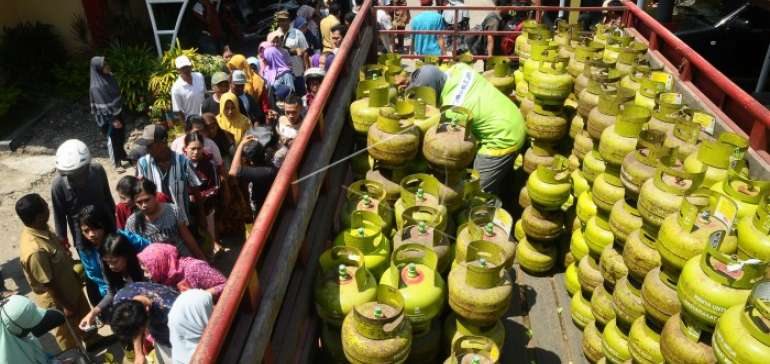
\includegraphics [width = 15cm]{gambar/antrian}
	\caption{Antrian Pembelian Tabung Gas LPG }
	\citep{antaraRiau}
	\label{antrian}
\end{figure}

\section{Rumusan Masalah}
Berdasarkan latar belakang yang telah diuraikan di atas, ada beberapa permasalahan yang akan dirumuskan pada penelitian ini, diantaranya:
\begin{enumerate}
	\item Apa saja kebutuhan yang diperlukan pengguna untuk melakukan pelaporan penyaluran gas LPG 3 Kg melalui aplikasi.
	\item Bagaimana aplikasi dapat melakukan validasi pada data pelaporan penyaluran gas LPG 3 Kg.
	\item Bagaimana aplikasi pelaporan penyaluran gas LPG 3 Kg dapat dipakai dengan mudah dan cepat.
\end{enumerate}

\newpage
\section{Tujuan Penelitian}
Tujuan dari penelitian ini adalah sebagai berikut:
\begin{enumerate}
	\item Memahami bagaimana pangkalan gas LPG melakukan pelaporan data penyaluran gas LPG 3 Kg.
	\item Merancang aplikasi yang dapat melakukan validasi pada data penyaluran gas LPG 3 Kg.
	\item Merancang aplikasi pelaporan penyaluran gas LPG 3 Kg berbasis android yang dapat dipakai dengan mudah dan cepat.
	\item Menghasilkan sebuah aplikasi yang layak dan telah sesuai dengan kebutuhan pengguna.
\end{enumerate}


\section{Manfaat Penelitian}
Manfaat dari penelitian ini adalah sebagai berikut:
\begin{enumerate}
	\item Meningkatkan efektivitas dalam semua proses terkait penyaluran tabung gas LPG 3 Kg.
	\item Menjadi bahan pembelajaran untuk mengembangkan sebuah \textit{mobile application} yang lebih baik dan berguna bagi masyarakat.
	\item Diharapkan aplikasi ini dapat mengawasi penyaluran tabung gas 3 Kg dan mempermudah masyarakat yang berhak untuk mendapatkan gas 3 Kg.
\end{enumerate}


% Baris ini digunakan untuk membantu dalam melakukan sitasi
% Karena diapit dengan comment, maka baris ini akan diabaikan
% oleh compiler LaTeX.
\begin{comment}
\bibliography{daftar-pustaka}
\end{comment}
